\documentclass{article}
\usepackage{amsmath}
\usepackage{amssymb}
\usepackage{changepage}
\usepackage{graphicx}
\title{Homework 1 Final Writeup}
\author{Michael Tang}
\begin{document}
\maketitle
\pagenumbering{arabic}
\begin{adjustwidth}{-2cm}{-2cm}

\section{Usage}
After running make, execute the program as follows in the working directory:\\
./spath [-s \textit{file}] [-p \textit{nthreads}] [-o \textit{outfile}] [-t \textit{step-by-step \& time file}]\\
where the italicized entries are the arguments that must come with each option.\\
-s is the required input file option, and must be followed by a filename. The file must be formatted as follows:
\begin{itemize}
	\item First number must be the number of vertices $N$.
	\item $N*N$ numbers must follow representing the $N \times N$ adjacency matrix of the graph.
	\item The only required text formatting is that each number is separated by whitespace.
	\item Numbers can only be as large, positive and negative, as the maximum and minimum numbers represented by your system's $int$ respectively.
\end{itemize}
-p is the optional parameter for number of threads, and if specified must be followed by an integer specifying the number of threads. Not specifying it will run serial mode, while specifying it will run parallel mode (even when $nthreads = 1$).\\
-o is the optional file path to write the program's output to. The path directed to will be opened in ``w'' mode, deleting any previous data in the file. If -o is not specified the program will write to stdout.\\
-t is the optional file path to write step-by-step output (currently muted to satisfy storage constraints, but used for correctness testing) and the time spent in Phase 2 in milliseconds, as outputted by stopwatch. Behavior is similar to -o except that the file will be opened in ``a'' mode, appending to any existing text in the file.\\
To enable utilization of the stopwatch object (the program will not compile correctly otherwise), stopwatch.h and stopwatch.c must be in a directory named "utils" that shares the same parent directory as the current working directory. It is already set up like this in my svn repository.

\section{Design Changes}
The design for preprocessing the $dist$ array has two significant changes: a distinct $edges$ array with the values of the initial adjacency matrix will not be given, and instead $dist$ will contain those values. During the parsing of the input file, parallelization will not be used, so Phase 1 is the same for both parallel and serial operation. Another less significant change is that $dist$ is now technically a 1-dimensional array, of length $N*N$ where $N$ is the number of vertices. This allows for easier access and printing treatment as well as possibly more cache hits due to the smaller address range needed, and only requires simple arithmetic for indexing.\\
For the parallel version of Phase 2, after the design review several significant changes were made to parallel operation design:
\begin{itemize}
	\item The plan to use mutexes for each element of the adjacency matrix has been eschewed. In class it was discussed that as long as all threads were operating at the same value of $k$ in Floyd-Warshall, then there are no race conditions.
	\item In order to reduce thread creation and joining overhead, instead of generating new threads every iteration of $k$ and waiting for all of them to join before proceeding to the next iteration, the final design generates the threads before beginning Floyd-Warshall.
	\item To maintain all threads at the same $k$, barrier synchronization is used via the $pthread_barrier$ interface. The barrier is placed at the end of a $k$ iteration, forcing all threads to wait until all threads are done with that iteration before proceeding.
\end{itemize}
The serial and the parallel operations utilize the same function $void* fl_wshl(void* tdata)$; this is the only significant change to the serial operation for Phase 2, that it uses the same function as parallel operation instead of having separate functions for parallel and serial operations. In serial operation barrier synchronization is disabled, and thread generation and closing is a concern outside of this shared function.

\section{Testing Results}
\subsection{Correctness}
To test serial correctness, the files test1.txt through test6.txt in mtang72-cs23010-spr-19/tests were used. The tests had to be easy enough to be verifiable by hand, but edge cases regarding length (test2, test3) and adjacencies (test6) were created.\\
For parallel correctness, the aforementioned test files as well as test7.txt and test1024.txt were used and the outputs compared with serial. For tests 1 through 7, 4 threads were used, and for test1024 64 threads were used. All final outputs matched the serial output. Step-by-step (at each $k$ iteration) outputs were also taken to test that invariant of correct step-by-step updating. A discrepancy was encountered here - according to these outputs sometimes, especially at higher values of $N$, the parallel operation would be exactly one step ahead. There is not a sure explanation of this, but the end result is the same.
\subsection{Performance}
The given stopwatch object was started before division of the code into parallel and serial operations, and ended right after. Thus it only measures time for Phase 2, which would maximize accuracy of speed comparisons because that is the only part where parallel and serial operations differ. Testing was done with SLURM, and all stopwatch outputs can be found in $/home/mtang72/slurm/hw1_out$ on the UChicago CS Linux computers.
\subsubsection{Overhead}
For overhead, times with serial and parallel ($nthreads = 1$) were taken for $N \in \{16,32,64,128,256,512,1024\}$. Below is a table of the data, where columns "Serial" and "Parallel" have data in milliseconds. Below that is a chart of runtime ratios for parallel 1-thread to serial versus number of vertices.\\
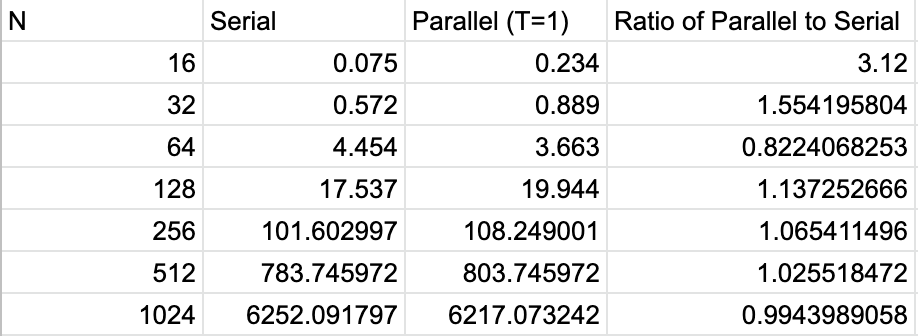
\includegraphics[width=\linewidth]{overheaddata.png}\\
\null\\
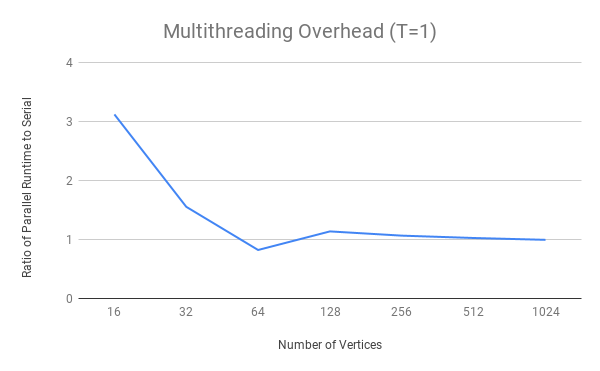
\includegraphics[width=\linewidth]{overhead.png}\\
Due to design changes thread creation overhead is no longer dependent on number of iterations within Floyd-Warshall. As a result, unlike what was hypothesized in the design draft but very much what I expected for this design, overhead was significant when number of vertices were low, while with larger number of vertices the overhead is negligible. In fact, sometimes the 1-thread parallel operation is faster than the serial operation. However, it is only ever faster by an insignificant margin which leaves room to conclude that it is likely caused by uncontrollable variables at runtime.
\subsubsection{Speedup}
For speedup, times with serial and parallel ($nthreads \in \{2,4,8,16,32,64\}$) were taken for $N \in \{16,32,64,128,256,512,1024\}$. Below is a table of the data, where column "Serial" is in milliseconds and columns "T=2" through "T=64" are ratios of serial runtime to parallel runtime. Below that is a chart of those runtime ratios, with each line representing a different amount of threads used.\\
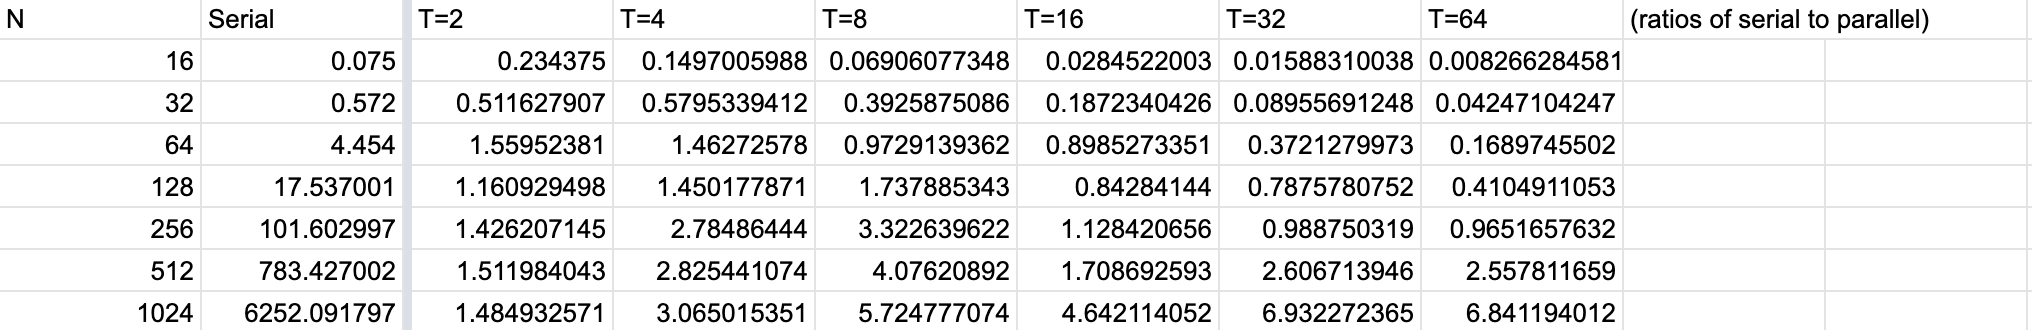
\includegraphics[width=\linewidth]{performancedata.png}\\
\null\\
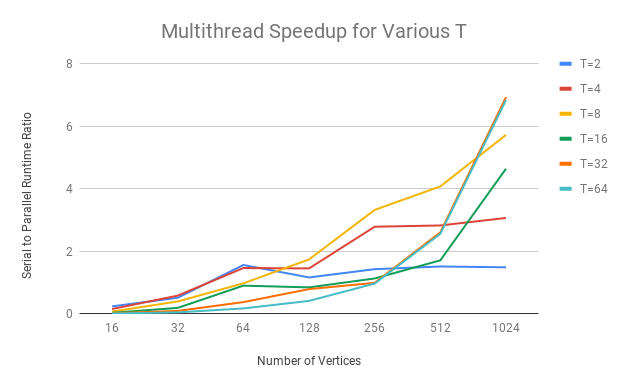
\includegraphics[width=\linewidth]{speedup.png}\\
Up to 6.9x speedup was achieved. Speedup notably fell at $T=16$ before rising again at $T=32$ then falling again. The first dip is likely because the SLURM node only had 14 cores available for usage, so at 16 threads certain cores had to share threads. The second rise could be because additional thread work was distributed more equitably among cores, and the second fall was likely because of additional burden given to each core that was already tasked, at 32 cores, to handle context switching between threads. The ratios at lower amounts of vertices are not very visible; below is the same graph, zoomed in to only the range between 16 and 64 vertices. Here we can see that at this lower number of vertices additional threads actually slowed the operation compared to serial ($ratio < 1$), and at 64 vertices only the 2 and 4 thread operations experience some speedup over serial. This can be explained by the overhead created by generating more threads, which becomes more negligible at larger numbers of vertices as we saw when testing overhead.\\
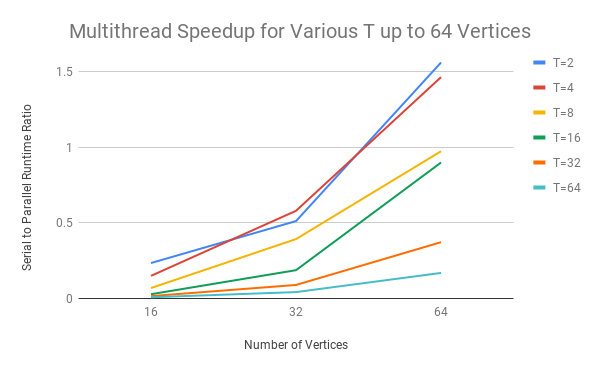
\includegraphics[width=\linewidth]{speeduplim.png}\\
Contrary to the hypothesis speedup never reached $1/T$ for any $T$, likely due to the overhead of thread creation and joining as well as of barrier synchronization. Additionally, at $T=16$ and above the program was not running truly parallel, as the need to handle more threads than there were cores forced serial context switching within cores.
\end{adjustwidth}
\end{document}